\documentclass[10pt,a4paper]{article}
\usepackage[utf8]{inputenc}
\usepackage{fullpage}
\usepackage{graphicx}
\usepackage{fancyhdr}
\usepackage{comment}
\usepackage{occi}
\setlength{\headheight}{13pt}
\pagestyle{fancy}

% default sans-serif
\renewcommand{\familydefault}{\sfdefault}

% no lines for headers and footers
\renewcommand{\headrulewidth}{0pt}
\renewcommand{\footrulewidth}{0pt}

% header
\fancyhf{}
\lhead{GWD-R}
\rhead{\today}

% footer
\lfoot{occi-wg@ogf.org}
\rfoot{\thepage}

% paragraphs need some space...
\setlength{\parindent}{0pt}
\setlength{\parskip}{1ex plus 0.5ex minus 0.2ex}

% some space between header and text...
\headsep 13pt

\setcounter{secnumdepth}{4}

% comments, temp stuff
\newcommand{\ralf}[1]{\textcolor{red}{Ralf: #1}}

\begin{document}

% header on first page is different
\thispagestyle{empty}

GWD-R \hfill  Thijs Metsch, Platform Computing\\
OCCI-WG \hfill  Andy Edmonds, Intel\\
\rightline {Ralf Nyrén, Aurenav}\\
\rightline {October 14, 2010}\\
\rightline {Updated: \today}

\vspace*{0.5in}

\begin{Large}
\textbf{Open Cloud Computing Interface - Core}
\end{Large}

\vspace*{0.5in}

\underline{Status of this Document}

This document provides information to the community regarding the
specification of the Open Cloud Computing Interface. Distribution is
unlimited.


\underline{Obsoletes}

This document obsoletes all previous versions of this document.

\underline{Copyright Notice}

Copyright \copyright Open Grid Forum (2009-2010). All Rights Reserved.

\underline{Trademarks}

OCCI is a trademark of the Open Grid Forum.

\underline{Abstract}

This document, part of a document series, produced by the OCCI working
group within the Open Grid Forum (OGF), provides a high-level
definition of a Protocol and API. The document is based upon
previously gathered requirements and focuses on the scope of important
capabilities required to support modern service offerings.


\newpage
\tableofcontents
\newpage

\section{Introduction}
The Open Cloud Computing Interface (OCCI) is a RESTful Protocol and
API for all kinds of management tasks. OCCI was originally initiated
to create a remote management API for IaaS%
\footnote{Infrastructure as a Service}
model-based services, allowing for the development of interoperable tools for
common tasks including deployment, autonomic scaling and monitoring.
%
It has since evolved into an flexible API with a strong focus on
interoperability while still offering a high degree of extensibility. The
current release of the Open Cloud Computing Interface is suitable to serve many
other models in addition to IaaS, including e.g.~PaaS and SaaS.

In order to be modular and extensible the current OCCI specification is
released as a suite of complimentary documents, which together form the complete
specification.
%
The documents are divided into three categories consisting of the OCCI Core,
the OCCI Renderings and the OCCI Extensions.
%
\begin{itemize}
\item The OCCI Core specification consists of a single document defining the
 OCCI Core Model. The OCCI Core Model can be interacted with {\em
 renderings} (including associated behaviours) and expanded through {\em extensions}.
\item The OCCI Rendering specifications consist of multiple documents each
 describing a particular rendering of the OCCI Core Model. Multiple renderings can
 interact with the same instance of the OCCI Core Model and will automatically support
 any additions to the model which follow the extension rules defined in OCCI
 Core.
\item The OCCI Extension specifications consist of multiple documents each
 describing a particular extension of the OCCI Core Model. The extension documents
 describe additions to the OCCI Core Model defined within the OCCI specification
 suite.
\end{itemize}
%
The current specification consist of three documents.
Future releases of OCCI may include additional rendering and extension
specifications. The documents of the current OCCI specification suite are:

\begin{description}
\item[OCCI Core] describes the formal definition of the the OCCI Core Model
\cite{occi:core}.
\item[OCCI HTTP Rendering] defines how to interact with the OCCI Core Model using the
RESTful OCCI API \cite{occi:http_rendering}. The document defines how the OCCI Core Model can
be communicated and thus serialised using the HTTP protocol.
\item[OCCI Infrastructure] contains the definition of the OCCI Infrastructure
extension for the IaaS domain \cite{occi:infrastructure}. The document defines
additional resource types, their attributes and the actions that can be taken
on each resource type.
\end{description}


\section{Notational Conventions}
All these parts and the information within are mandatory for
implementors (unless otherwise specified). The key words "MUST", "MUST
NOT", "REQUIRED", "SHALL", "SHALL NOT", "SHOULD", "SHOULD NOT",
"RECOMMENDED", "MAY", and "OPTIONAL" in this document are to be
interpreted as described in RFC 2119 \cite{rfc2119}.

\textbf{Andy: we need to state that this document as part of the current document set,
supersedes all previous documents.}


\section{OCCI Core}
The Open Cloud Computing Interface is a boundary protocol and API
that acts as a service front-end to a provider's internal management
framework. Figure~\ref{fig:placement} shows OCCI's place in a
provider's architecture.
\begin{figure}[h]
	\centering
	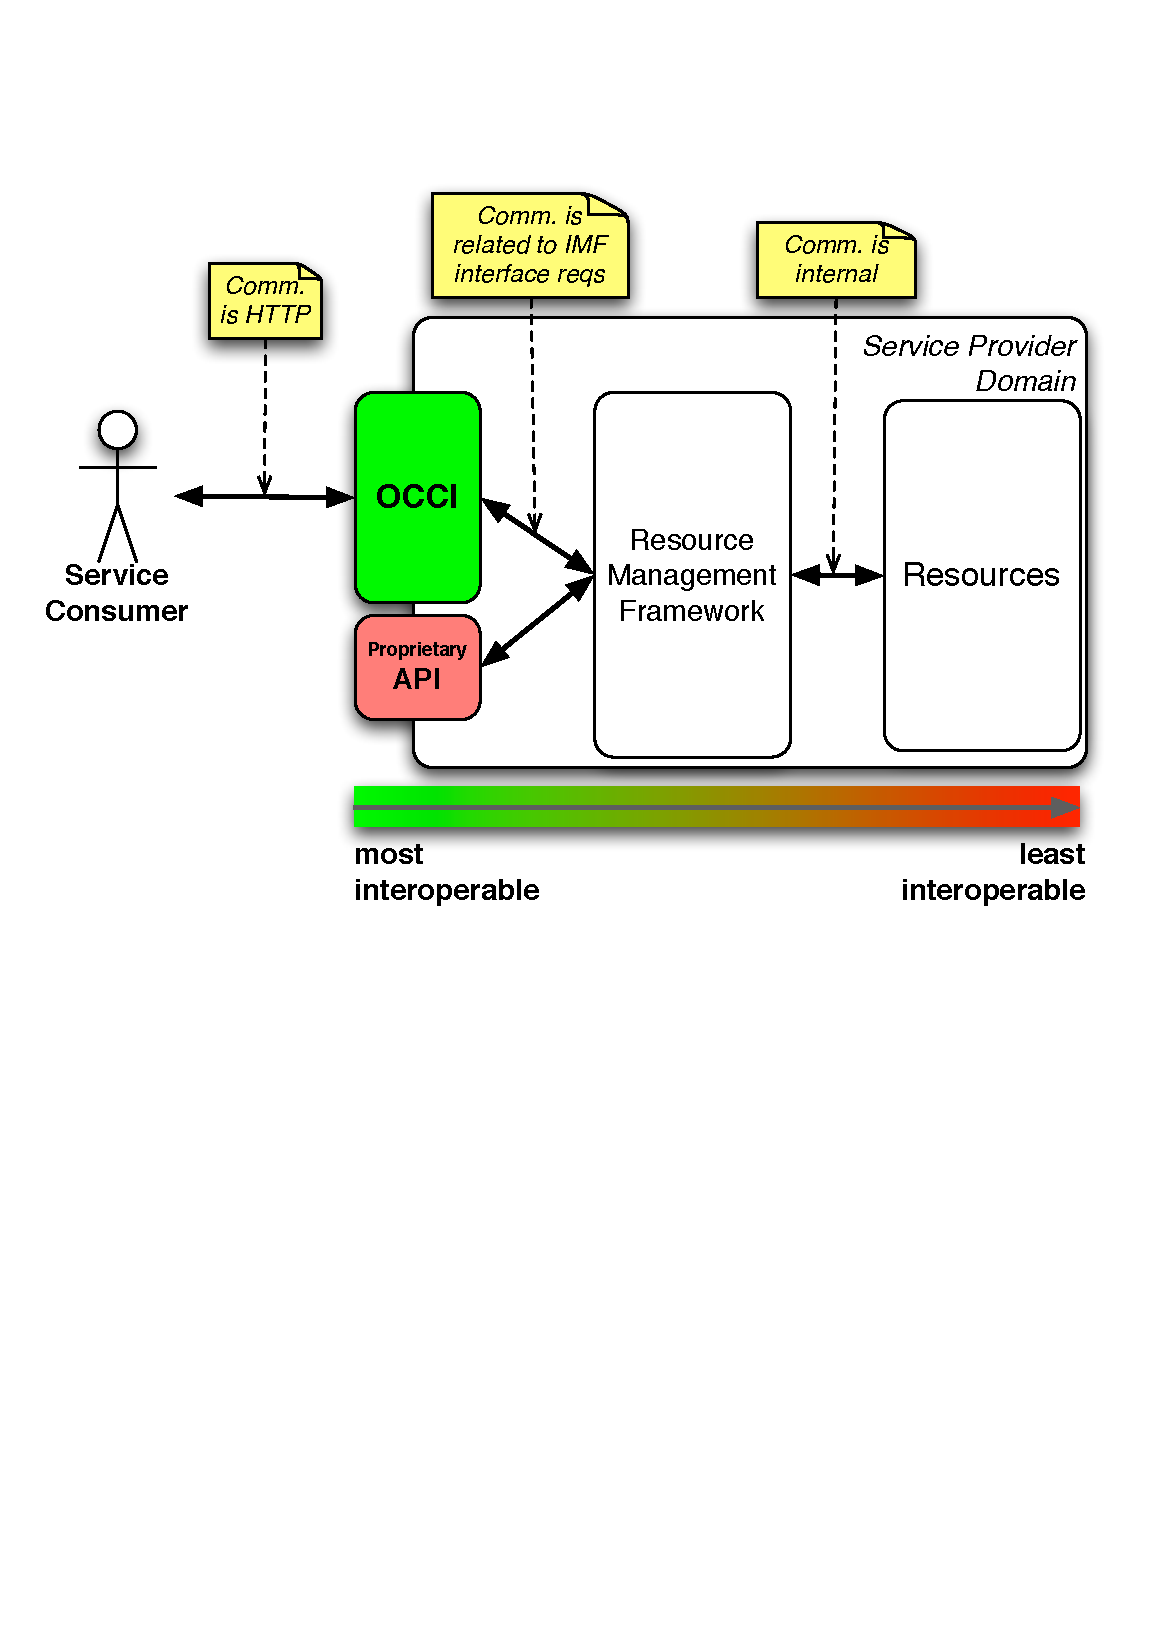
\includegraphics[scale=0.5]{figs/occi-intro.pdf}
	\caption{OCCI's place in a provider's architecture}
	\label{fig:placement}
\end{figure}
Service consumers can be both end-users and other system instances. OCCI is
suitable for both cases. The key feature is that OCCI can be used as a
management API for all kinds of resources while at the same time maintaining a
high level of interoperability.

This document, the OCCI Core specification, defines the OCCI Core Model. This
model is the core of the specification suite and it can be interacted with 
by renderings (including associated behaviours) and expanded 
through extensions. In itself, the core model is only useful
for a very limited set of use cases. However, it provides the basis for
renderings and extensions to build upon.

\section{OCCI Core Model}
The OCCI Core Model defines a representation of instance types which can be
manipulated through an OCCI Rendering implementation. 
It is an abstraction of real-world 
resources, including the means to identify, classify, associate 
and extend those resources. 

A fundamental feature of the OCCI Core Model is that it can be extended in such a
way that any extension will be discoverable and visible to an OCCI client at
run-time. An OCCI client can connect to an OCCI implementation using an
extended OCCI Core Model, without knowing anything in advance, and still be
able to discover and understand, at run-time, the various \hl{Resource} and \hl{Link} sub-types
supported by that implementation. What \hl{Mixin}s are supported is also discoverable in the 
same fashion. For example, a web-based OCCI client could easily be reused as the 
management tool for a wide variety of services.

The OCCI Core Model can be extended through inheritance but also
using a ``mix-in'' like concept.
\begin{quote}
Mixins first appeared in the Symbolics' 
object-oriented Flavors~\cite{Moon:1986:flavors}
system (developed by Howard Cannon), which was an 
approach to object-orientation used in Lisp Machine Lisp.%
\footnote{http://en.wikipedia.org/wiki/Mixin.}
\end{quote}
%
The mix-in model only applies at the instance
level, i.e.~the ``object level'', and thereby differs from the more common uses
of the mix-in concept. A mix-in in OCCI can never be applied to a type, only to
an instance.

\subsection{Overview}

The UML class diagram shown in figure~\ref{fig:occi_model} gives an overview of
the OCCI Core Model. It must be noted that the UML diagram in itself is not a
complete definition of the model. The diagram is merely provided as an overview
to help understanding the model. 

\begin{figure}[!h]
{\centering \resizebox*{0.9\columnwidth}{!}{\rotatebox{270}
      {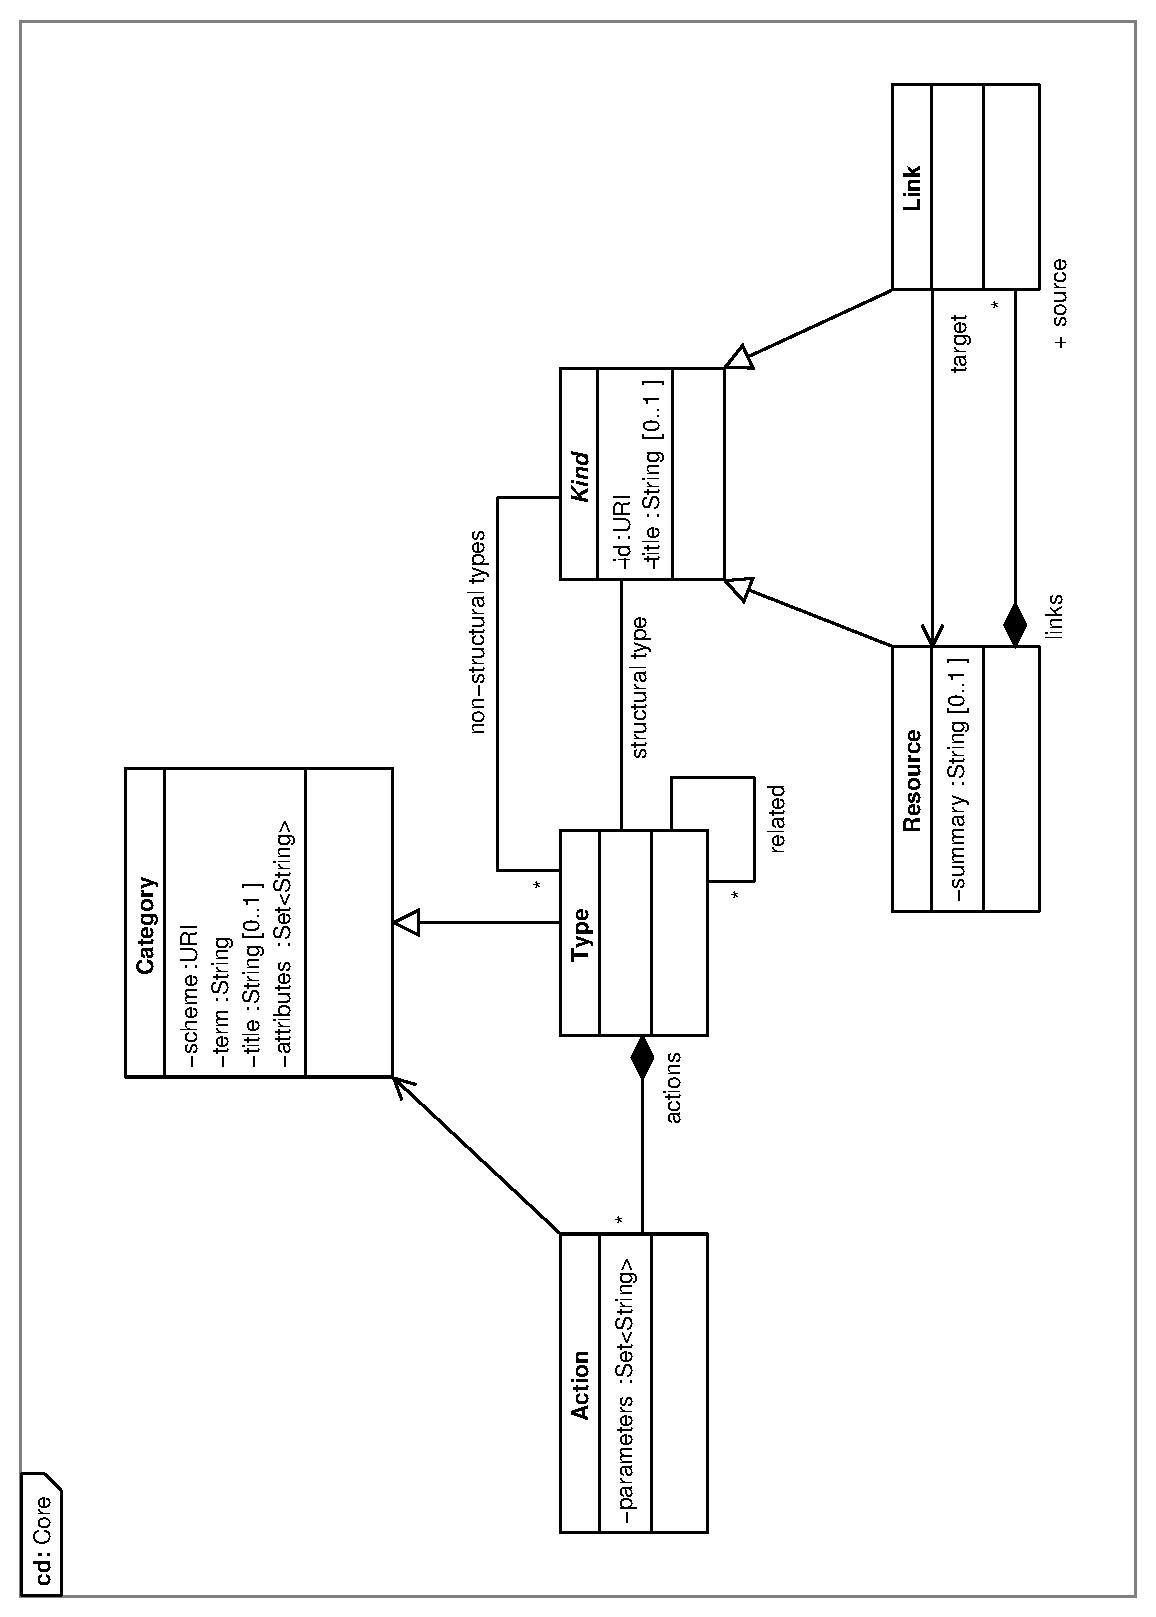
\includegraphics{figs/core_model.pdf}}} \par}
\caption{UML class diagram of the OCCI Core Model. The diagram provides an
overview of the OCCI Core Model but is not a standalone definition thereof}
\label{fig:occi_model}
\end{figure}

The heart of the OCCI Core Model is the \hl{Resource} type. Any resource exposed
through OCCI is a \hl{Resource} or a sub-type thereof.
A resource can be e.g.~a virtual machine, a job in a job submission system, a
user, etc.
%
The \hl{Resource} type contains a number of common attributes that
\hl{Resource} sub-types inherit. The \hl{Resource} type is
complemented by the \hl{Link} type which associates one \hl{Resource} instance
with another.
%
The \hl{Link} type contains a number of common attributes that
\hl{Link} sub-types inherit.

\hl{Entity} is an abstract type which both \hl{Resource} and \hl{Link} inherit.
Each sub-type of \hl{Entity} is identified by a unique \hl{Kind} instance.
%

The \hl{Kind} type is the core of the type classification
system built into the OCCI Core Model. \hl{Kind} is a specialisation of
\hl{Category} and introduces additional resource capabilities in terms of \hl{Action}s.
An \hl{Action} represent an invocable operation applicable to a resource
instance.

The last type defined by the OCCI Core Model is the \hl{Mixin} type. An instance of
\hl{Mixin} can be associated with a resource instance, i.e.~a sub-type of
\hl{Entity}, to ``mix-in'' additional resource capabilities at run-time.
%
For compliance with OCCI Core, all of the types defined in the OCCI Core Model MUST
be implemented.  The following sections of the specification contain the formal
definition of the OCCI Core Model.

\subsection{Terms and definitions}
Section \ref{sec:glossary} provides a glossary of all terms and definitions with
a specific meaning to the OCCI specification suite. However, for reader
convenience, a sub-set of the glossary is provided here as well. The following
terminology have specific meaning in the OCCI context:
\begin{description}
\item[concrete type/sub-type] A concrete sub-type is a type that can be instantiated.
\item[mix-in] An instance of the \hl{Mixin} type associated with a {\bf resource
 instance}. The ``mix-in'' concept as used by OCCI {\em only} applies to
 instances, never to \hl{Entity} types.
\item[OCCI base type(s)] The OCCI base types are \hl{Entity}, \hl{Resource},
 \hl{Link} and \hl{Action}.
\item[resource capabilities] Resource capabilities refer to attributes and
 \hl{Action}s exposed by a resource instance.
\item[resource instance] An instance of a sub-type of \hl{Entity}. The OCCI
 model defines two sub-types of \hl{Entity}, the \hl{Resource} type and the
 \hl{Link} type.  However, the term {\bf resource instance} is defined to
 include any instance of a {\em sub-type} of \hl{Resource} or \hl{Link} as
 well.
\item[type] A {\bf type} refer to one of those defined by the OCCI Core Model.
 The OCCI Core Model types are \hl{Category}, \hl{Kind}, \hl{Mixin},
 \hl{Action}, \hl{Entity}, \hl{Resource} and \hl{Link}.
\end{description}

\subsection{Mutability}

Attributes of an OCCI Core Model type instance are
either client mutable or client immutable. If an attribute is noted to
be mutable this MUST be interpreted that a client can create an
instance that is parametrised by the attribute. Likewise, if
an attribute is mutable, a client can update that instance's
mutable attribute value and the server side MUST support this. If an
attribute is marked as immutable, it indicates that the server side
implementation MUST manage these exclusively. Immutable attributes
MUST NOT be modifiable by clients under any circumstance.

\subsection{Classification and Identification}
\label{sec:classification}
The OCCI Core Model provides a built-in type classification system allowing for safe
extension towards domain-specific usage (e.g. infrastructure). This system is the OCCI type system
and offers the means to be easily and transparently (i.e. no format translation required) exposed over either a text or binary based protocol.
%
The classification system can be summarised with the following key features:
\begin{itemize}
\item Each OCCI base type and extension thereof is assigned a unique type
 identifier (a \hl{Kind} instance), which allow for dynamic discovery of
 available types. All \hl{Entity} sub-types, including core model extensions, are assigned
 a unique \hl{Kind} instance.
\item The inheritance structure of \hl{Entity}, \hl{Resource} and \hl{Link} is
 client discoverable. This also applies to any sub-type of \hl{Resource} and
 \hl{Link} and therefore an OCCI client can discover the type inheritance structure
 used by a particular OCCI implementation. The discovery of the inheritance
 structure is made possible through the relationship of \hl{Kind} instances.
\item The classification system allows \hl{Mixin} instances to be associated
 to resource instances in order to assign additional resource capabilities in terms of
 attributes and \hl{Action}s at run-time.
\item Tagging of resource instances is supported through the association
 of \hl{Mixin} instances. A tag is simply a \hl{Mixin} instance which define no
 additional resource capabilities.
\item A collection of associated resource instances is implicitly defined for
 each \hl{Kind} and \hl{Mixin} instance. I.e.~all resource instances associated
 with a particular \hl{Kind} or \hl{Mixin} instance form a collection.
\end{itemize}

\subsubsection{Category}
\label{sec:category}
The \hl{Category} type is the basis of the type
identification mechanism used by the
OCCI classification system. It MUST be implemented. Instances of the
\hl{Category} type itself are only used to identify \hl{Action} types. All
other uses of \hl{Category} properties are managed through its sub-types
\hl{Kind} and \hl{Mixin}.
%
Table~\ref{tbl:category} defines the attributes the \hl{Category} type MUST
implement to be compliant.

\mytablefloat{\label{tbl:category}Attributes defined for the \hl{Category} type}{
\begin{tabular}{llllp{2.7in}}
\toprule
Attribute & Type & Multiplicity & Client Mutability & Description \\
\colrule
term & String & 1 & Immutable & Unique identifier of the \hl{Category} instance within the categorisation scheme. \\
scheme & URI & 1 & Immutable & The categorisation scheme. \\
title & String & 0..1 & Immutable & The display name of an instance. \\
attributes & String & 0..* & Immutable & The set of resource attribute names defined by the \hl{Category} instance. \\
\botrule
\end{tabular}
}

A \hl{Category} instance is uniquely identified by concatenating the
categorisation scheme with the category term,
e.g.~\textit{http://example.com/category/scheme\#term}.
This is done to enable discovery of \hl{Category} definitions in text based
renderings such as HTTP. All renderings MUST make use of and understand
concatenated unique type identifiers of \hl{Category} instances.
%
Sub-types of \hl{Category} such as \hl{Kind} and \hl{Mixin} inherit this property.

The categorisation schemes defined in the OCCI specification all use the
\textit{http://schemas.ogf.org/occi/} base URL. This base URL is reserved for
OCCI an MUST NOT be used by service provider extensions.

A \hl{Category} instance%
\footnote{Also applies to \hl{Kind} and \hl{Mixin} instances.}
define the {\em names} of the attributes exposed by any instance associated
with the \hl{Category}.  For example a ``resize'' \hl{Action} having a {\tt
size} attribute would have an identifying \hl{Category} with \hl{Category}.{\tt
attributes = [ size ]}.

\subsubsection{Kind}
\label{sec:kind}

The \hl{Kind} type, together with the \hl{Mixin} type, defines the
classification system of the OCCI Core Model. It MUST be implemented. The \hl{Kind}
type represents the type identification mechanism for all \hl{Entity} types present in
the model.

A unique \hl{Kind} {\em instance} MUST be assigned to each and every
\hl{Entity} sub-type defined in an OCCI implementation.
%
Every instance of \hl{Kind} represents a unique type identifier for a
particular sub-type of \hl{Entity}.  Consequently, when an \hl{Entity} sub-type
is instantiated the resource instance MUST be associated with its type
identifier, i.e.~the \hl{Kind} instance.  A resource instance MUST remain
associated with its \hl{Kind} instance throughout its lifetime.
%
For example an instance of \hl{Resource} MUST always be associated with the
\hl{Kind} instance which identifies the \hl{Resource} {\em type}.

In the initial instantiation of the OCCI Core Model, with no core model
extensions, three instances of \hl{Kind} will be present: one for \hl{Entity},
another for \hl{Resource} and the last one for \hl{Link}. 

\mytablefloat{\label{tbl:kind}Attributes defined for the \hl{Kind} type}{
\begin{tabular}{llllp{2.7in}}
\toprule
Attribute & Type & Multiplicity & Client Mutability & Description \\
\colrule
actions & \hl{Action} & 0..* & Immutable & Set of \hl{Action}s defined by the \hl{Kind} instance. \\
related & \hl{Kind} & 0..* & Immutable & Set of related \hl{Kind} instances. \\
entity\_type & \hl{Entity} & 1 & Immutable & \hl{Entity} type uniquely identified by the \hl{Kind} instance. \\
entities & \hl{Entity} & 0..* & Immutable & Set of resource instances, i.e.~\hl{Entity} sub-type instances. Resources instantiated from the \hl{Entity} sub-type which is uniquely identified by this \hl{Kind} instance. \\
\botrule
\end{tabular}
}
The \hl{Kind} type inherits the \hl{Category} type. To be compliant the \hl{Kind}
type MUST implement the attributes defined in table~\ref{tbl:kind} and the inherited
attributes defined in table~\ref{tbl:category}. The following rules apply to all
instances of the \hl{Kind} type:
\begin{itemize}
\item A unique \hl{Kind} instance MUST be assigned to each and every sub-type
 of \hl{Entity}, including \hl{Entity} itself.
\item A \hl{Kind} instance MUST expose the attribute names of the \hl{Entity}
 sub-type it identifies. The attribute names are exposed through the ``{\tt
 attributes}'' attribute inherited from \hl{Category}. E.g.~the \hl{Kind}
 instance identifying the \hl{Link} type has \hl{Kind}.{\tt attributes =
 [ source, target ]}.
\item A \hl{Kind} instance MUST expose the \hl{Action}s defined for its
 \hl{Entity} sub-type. \hl{Action}s are exposed through the \hl{Kind}.{\tt
 actions} attribute which represent the association between a \hl{Kind}
 instance and the \hl{Action}s it defines.
\item A \hl{Kind} instance MUST be related, either directly or indirectly, to
 the \hl{Kind} instance of \hl{Entity},
 i.e. \textit{http://schemas.ogf.org/occi/core\#entity}.
 The \hl{Kind}.{\tt related} attribute represent the relationship to another
 \hl{Kind} instance.
\item If type {\bf B} inherits type {\bf A}, where {\bf A} is a sub-type of
 \hl{Entity}, the \hl{Kind} instance of {\bf B} MUST be directly related to the
 \hl{Kind} instance of {\bf A}. See Kind Relationships below.
\end{itemize}

\paragraph*{Kind Relationships}
\hl{Kind} relationships are defined through the {\tt related} attribute present
in every \hl{Kind} instance. The {\tt related} attribute define which other
\hl{Kind} instances a particular \hl{Kind} is related to.

A \hl{Kind} instance identify a unique type, either the \hl{Entity} type itself
or a sub-type thereof.  Each \hl{Kind} instance MUST be related to the
\hl{Kind} of the parent type.
%
The OCCI base types \hl{Resource} and \hl{Link} both extend \hl{Entity} and
therefore their identifying \hl{Kind} instances MUST be related to \hl{Kind}
assigned to the \hl{Entity} type.
%
These rules imply a hierarchy of related \hl{Kind} instances. The \hl{Kind}
relationships thus mirror the type inheritance structure of the OCCI Core
Model and any extension thereof.

\begin{figure}[!h]
{\centering \resizebox*{0.9\columnwidth}{!}{\rotatebox{0}
      {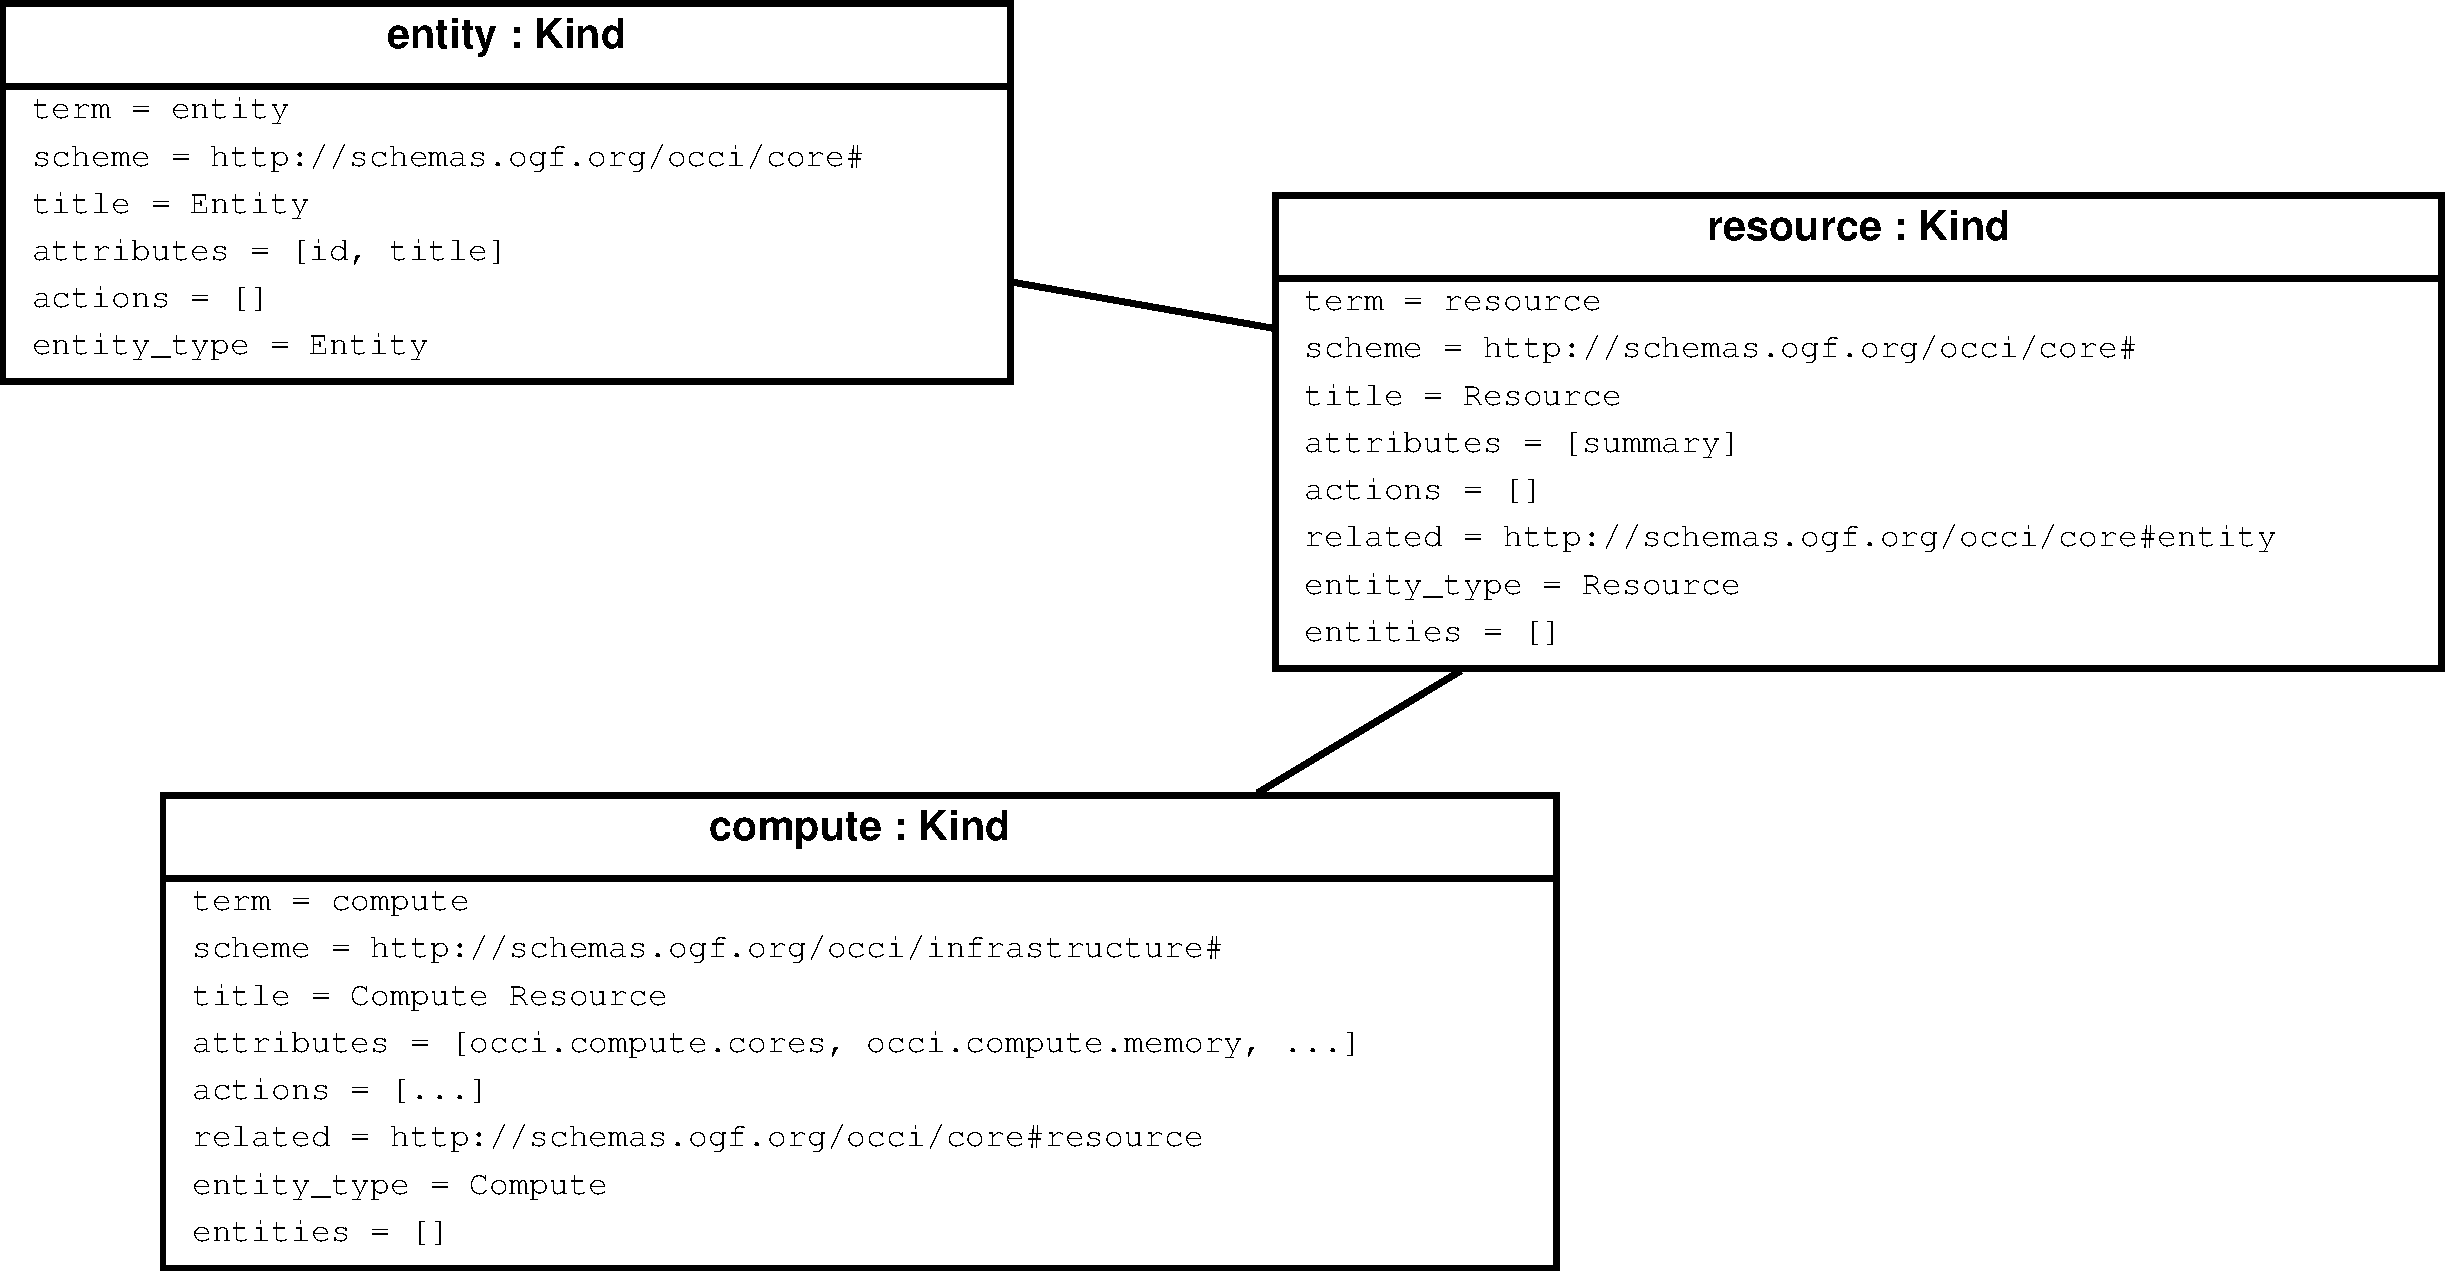
\includegraphics{figs/kind_relationships.pdf}}} \par}
  \caption{Object diagram illustrating the \hl{Kind} instances involved for the
  \hl{Entity}, \hl{Resource} and \hl{Compute} types. The \hl{Compute} type is an
  extension to the OCCI Core Model defined in the OCCI Infrastructure
  document~\cite{occi:infrastructure}.}
  \label{fig:kind_relationships}
\end{figure}

Figure~\ref{fig:kind_relationships} illustrates the relationship of the \hl{Kind}
instances assigned to the \hl{Entity}, \hl{Resource} and \hl{Compute}%
\footnote{The \hl{Compute} type is defined in the OCCI Infrastructure
 document~\cite{occi:infrastructure}.}
types.
%
\hl{Compute} inherits \hl{Resource} and therefore the \hl{Kind} instance
assigned to \hl{Compute} is related to the \hl{Kind} instance of \hl{Resource}.
The same applies to the \hl{Resource} type which inherit \hl{Entity}.
%
As can be seen in figure~\ref{fig:kind_relationships} the \hl{Kind} instance
relationships mirror the inheritance structure of the types.

\subsubsection{Mixin}
The \hl{Mixin} type complements the \hl{Kind} type in defining the
OCCI Core Model type classification system. It MUST be implemented. The \hl{Mixin}
type represent an extension mechanism, which allow new resource capabilities to
be added to resource instances both at creation-time and/or run-time.

A \hl{Mixin} {\em instance} can be associated with any existing resource
instance and thereby add new resource capabilities, i.e.~attributes and
\hl{Action}s, to the resource instance. However, a \hl{Mixin} can never be
applied to a type.
In the initial instantiation of the OCCI Core Model, with no extensions, no
\hl{Mixin} instances are present.

A \hl{Mixin} instance MAY be associated with any resource instance, either at
instance creation-time or at run-time. Although the OCCI Core Model has no such
restrictions, an OCCI implementation MAY impose restrictions on which resource
instances can be associated with a particular \hl{Mixin} instance.
%
When a client attempts to associate a \hl{Mixin} instance to a resource at a
stage not supported by a particular provider's OCCI implementation, the
provider MUST notify the client it has issued a bad request.
%
For example a ``geographical location'' \hl{Mixin} might by applicable to all
resource instances while a ``bandwidth'' \hl{Mixin} may only applicable
to resources instantiated from the \hl{Network}%
\footnote{The \hl{Network} type is defined in OCCI Infrastructure~\cite{occi:infrastructure}.}
type. Such restrictions, if not otherwise stated, are up to the provider to
implement.

\mytablefloat{\label{tbl:mixin}Attributes defined for the \hl{Mixin} type}{
\begin{tabular}{llllp{2.7in}}
\toprule
Attribute & Type & Multiplicity & Client Mutability & Description \\
\colrule
actions & \hl{Action} & 0..* & Immutable & Set of \hl{Action}s defined by the \hl{Mixin} instance. \\
related & \hl{Mixin} & 0..* & Immutable & Set of related \hl{Mixin} instances. \\
entities & \hl{Entity} & 0..* & Mutable & Set of resource instances, i.e.~\hl{Entity} sub-type instances, associated with the \hl{Mixin} instance. \\
\botrule
\end{tabular}
}
The \hl{Mixin} type inherits the \hl{Category} type. To be compliant the
\hl{Mixin} type MUST implement the attributes defined in table~\ref{tbl:mixin}
and the inherited attributes defined in table~\ref{tbl:category}. The following
rules apply to all instances of the \hl{Mixin} type:
\begin{itemize}
\item A \hl{Mixin} instance MUST only be associated with resource
 {\em instances}, not types, either at creation-time or run-time.
\item A \hl{Mixin} instance MAY introduce additional resource attributes when
 applied to a resource instance. The names of those attributes MUST be exposed
 through the \hl{Mixin}.{\tt attributes} attribute inherited from
 \hl{Category}.  E.g.~a Location \hl{Mixin} defining the ``com.example.location''
 attribute MUST have Location.{\tt attributes = [ com.example.location ]}.
\item A \hl{Mixin} instance MAY define \hl{Action}s which will be made
 applicable to any resource instance associated with the \hl{Mixin}.
 \hl{Action}s defined by a \hl{Mixin} are exposed through the \hl{Mixin}.{\tt
 actions} attribute which represent the association between a \hl{Mixin}
 instance and the \hl{Action}s it defines.
\item A \hl{Mixin} instance MAY be related to another \hl{Mixin} instance.
 If \hl{Mixin} {\bf B} is related to \hl{Mixin} {\bf A}, any resource instance
 associated with \hl{Mixin} {\bf B} will receive the resource capabilities
 defined by both \hl{Mixin} {\bf B} and \hl{Mixin} {\bf A}.
 %
 See Mixin Relationships below.
\item A \hl{Mixin} instance defining no additional resource capabilities is
 considered to be a tag.
\item A \hl{Mixin} instance applied a resource instantiation time MAY cause
 additional provider-defined side-effects to occur, side-effects not visible
 through the OCCI discovery mechanism. Templates that pre-populate certain
 attributes of a resource instance SHOULD be implemented using such \hl{Mixin}
 instances.
\end{itemize}

\paragraph*{Mixin Relationships}

A \hl{Mixin} instance MAY be related to another \hl{Mixin} instance for
type classification purposes. For example a set of operating system templates,
implemented as \hl{Mixin} instances, could be related to an ``OS-template''
\hl{Mixin} in order to help identification.

Attributes and \hl{Action}s defined by different \hl{Mixin} instances are
combined when \hl{Mixin} relationships are present. Therefore a resource
instance associated with a particular \hl{Mixin} will receive the additional
capabilities defined by any related \hl{Mixin} instances as well as those
defined by the \hl{Mixin} associated.

\subsubsection{Resource Instantiation}
\label{sec:instantiation}
To create a resource instance a client MUST supply the concrete
\hl{Entity} sub-type by a submitting a reference to the type-identifying \hl{Kind}.
The reference MUST consist of the term and categorisation scheme which
uniquely identify the \hl{Kind} instance, see section~\ref{sec:category}.
All OCCI implementations MUST understand these requests.

A client MAY also submit any number of references to \hl{Mixin} instances to be
associated with the resource to be created. A \hl{Mixin} reference submitted by
a client MUST consist of the term and categorisation scheme which identify
the \hl{Mixin} instance, see section~\ref{sec:category}. 

Associating a \hl{Mixin} at resource
instantiation time MAY have additional provider defined side-effects,
side-effects not visible through the OCCI discovery mechanism. Templates that
pre-populate certain attributes of a resource instance SHOULD be implemented
using such \hl{Mixin} instances.

\subsubsection{Collections}
\label{sec:collection}
One or more resource instances associated with the same \hl{Kind} or \hl{Mixin}
instance, automatically form a collection.
Each \hl{Kind} and \hl{Mixin} instance in the system identifies a collection
consisting of all different resource instances associated with the \hl{Kind} or
\hl{Mixin}.

A resource instance is always a member of the collection indicated by the
\hl{Entity} sub-type's unique \hl{Kind} instance. A \hl{Kind} instance maintains
the collection of all resource instances (of the type identified by the
\hl{Kind}).
%
Since a \hl{Mixin} instance can be associated to any resource instance, a
collection can contain resource instances of different \hl{Entity} sub-types.
%
For example, an instance of the \hl{Resource} type will always be associated
to the \hl{Kind} instance
\textit{http://scheme.ogf.org/occi/core\#resource} and thus part of the
collection implied by that \hl{Kind} instance.
\begin{description}
\item[Adding a resource instance] to a collection is accomplished by associating the
 resource instance to the corresponding \hl{Mixin} instance.
\item[Removing a resource instance] from a collection is accomplished by disassociating
 the resource instance from the corresponding \hl{Mixin} instance.
\end{description}
%
An OCCI implementation MUST allow a client to navigate collections. The
following basic navigation operations MUST be supported:
\begin{itemize}
\item Retrieve the whole collection.
\item Retrieve a specific item in a collection.
\item Retrieve a subset of a collection.
\end{itemize}
%
The details of collection navigation is rendering specific.

\subsubsection{Discovery}
\label{sec:discovery}
An OCCI client MUST be able to discover all instances of \hl{Kind}, \hl{Mixin}
and \hl{Category} a particular service provider's OCCI implementation has
defined. By examining these instances a client MUST be able to, at a minimum,
deduce the following information:
\begin{itemize}
\item The \hl{Entity} sub-types available from the service provider,
 including core model extensions. This information is provided through the
 \hl{Kind} instances of the OCCI implementation.
\item The attributes defined for each \hl{Entity} sub-type. The identifying
 \hl{Kind} instance provide this information.
\item The invocable operations, i.e.~\hl{Action}s, defined for each \hl{Entity}
 sub-type. The identifying \hl{Kind} instance provide this information.
\item Any \hl{Mixin} instances that can be associated to resource instances.
\item Additional capabilities defined by a particular \hl{Mixin} instance,
 i.e.~attributes and \hl{Action}s.
\end{itemize}
The above requirements comprise the OCCI discovery mechanism. It MUST be
implemented.
%
The details of exactly how the \hl{Category}, \hl{Kind} and \hl{Mixin}
instances are exposed to an OCCI client is specific to the particular rendering
used.
The relevant details can be found in the OCCI Rendering documents.


\subsection{The OCCI Core Base Types}
\label{sec:base_types}
The following sections describe the OCCI base types defined by the OCCI Core Model.
The base types are \hl{Entity}, \hl{Resource}, \hl{Link} and \hl{Action}. All
base types MUST be implemented.

\subsubsection{Entity}
\label{sec:entity}
The \hl{Entity} type is an abstract type of the \hl{Resource} type and the
\hl{Link} type. It MUST be implemented.
%
Table~\ref{tbl:entity} defines the attributes the \hl{Entity} type MUST implement to
be compliant.
%
\mytablefloat{\label{tbl:entity}Attributes defined for the \hl{Entity} type.}{
\begin{tabular}{lllp{1.3cm}p{1.0cm}p{7cm}}
\toprule
Attribute & Type & Multiplicity & Client Mutability & Discover\-able & Description \\
\colrule
id & URI & 1 & Immutable & Yes & A unique identifier (within the service provider's name-space) of the \hl{Entity} sub-type instance. \\
title & String & 0..1 & Mutable & Yes & The display name of the instance. \\
kind & \hl{Kind} & 1 & Immutable & No & The \hl{Kind} instance uniquely identifying the \hl{Entity} sub-type of the resource instance. \\
mixins & \hl{Kind} & 0..* & Mutable & No & The \hl{Mixin} instances associated to this resource instance. Consumers can expect the attributes and \hl{Action}s of the associated \hl{Mixin}s to be exposed by the instance. \\ 
\botrule
\end{tabular}}

\hl{Entity} enforces for all sub-types a required \texttt{id} attribute and an
optional \texttt{title} attribute.
%
Every sub-type of \hl{Entity} MUST be assigned a \hl{Kind} instance, see
section~\ref{sec:kind}.
%
\mytablefloat{\label{tbl:entity_kind}The \hl{Kind} instance assigned to the \hl{Entity} type.}{
\begin{tabular}{ll}
\toprule
Attribute & Value \\
\colrule
term & entity \\
scheme & {\tt http://schemas.ogf.org/occi/core\#} \\
title & Entity type \\
attributes & id, title \\
actions & -- \\
\botrule
\end{tabular}}
%
\hl{Entity} itself is assigned the \hl{Kind} instance
\textit{http://schemas.ogf.org/occi/core\#entity} for type identification, see
table~\ref{tbl:entity_kind}.
%
Being an abstract type \hl{Entity} itself can never be instantiated.
%
An \hl{Entity} sub-type instance, a resource instance, MAY be associated with
one or more \hl{Mixin} instances.

An \hl{Entity} sub-type instance MUST expose its identifying \hl{Kind} instance
and any associated \hl{Mixin} instances together with the attributes and
\hl{Action}s defined by them.

\subsubsection{Resource}
\label{sec:resource}
The \hl{Resource} type inherits \hl{Entity} and describes a concrete resource that
can be inspected and manipulated. It represents a general object in the OCCI
model and MUST be implemented. A \hl{Resource} is suitable to represent real
world resources, e.g. virtual machines, networks, services, etc.~through specialisation.
%
The \hl{Resource} type MUST implement all attributes inherited from \hl{Entity}
as well as the attributes defined in table~\ref{tbl:resource} in order
to be compliant.

\mytablefloat{\label{tbl:resource}Attributes defined for the \hl{Resource} type.}{
\begin{tabular}{llllp{8cm}}
\toprule
Attribute & Type & Multiplicity & Client Mutability & Description \\
\colrule
summary & String & 0..1 & Mutable & A summarising description of the \hl{Resource} instance.\\
links & \hl{Link} & 0..* & Mutable & A set of \hl{Link} compositions. Being a composite relation the removal of a \hl{Link} from the set MUST also remove the \hl{Link} instance.\\
\botrule
\end{tabular}
}

The \hl{Resource} type is assigned the \hl{Kind} instance
\textit{http://schemas.ogf.org/occi/core\#resource}, see
table~\ref{tbl:resource_kind}.
%
\mytablefloat{\label{tbl:resource_kind}The \hl{Kind} instance assigned to the \hl{Resource} type.}{
\begin{tabular}{ll}
\toprule
Attribute & Value \\
\colrule
term & resource \\
scheme & {\tt http://schemas.ogf.org/occi/core\#} \\
title & Resource \\
attributes & summary \\
actions & -- \\
\botrule
\end{tabular}}

\hl{Resource} enforces the inheritance of a set of common attributes into
sub-types. Moreover, it introduces relationships to other \hl{Resource}
instances through instances of the \hl{Link} type.
%
The \hl{Resource} type is the first of three entry points to extend the OCCI Core
Model, see section~\ref{sec:extensibility}.

\subsubsection{Link}
\label{sec:link}
An instance of the \hl{Link} type defines a base association between two
\hl{Resource} instances. It MUST be implemented. A \hl{Link} instance indicates
that one \hl{Resource} instance is connected to another.
%
The \hl{Link} type MUST implement all attributes inherited from the
\hl{Entity} type together with the attributes defined in table~\ref{tbl:link}
in order to be compliant.
%
\mytablefloat{\label{tbl:link}Attributes defined for the \hl{Link} type.}{
\begin{tabular}{llllp{7.5cm}}
\toprule
Attribute & Type & Multiplicity & Client Mutability & Description \\
\colrule
source & \hl{Resource} & 1 & Mutable & The \hl{Resource} instances the \hl{Link} instance originates from.\\
target & \hl{Resource} & 1 & Mutable & The \hl{Resource} instances the \hl{Link} instance points to.\\
\botrule
\end{tabular}}

The \hl{Link} type is assigned the \hl{Kind} instance
\textit{http://schemas.ogf.org/occi/core\#link}.
%
\mytablefloat{\label{tbl:link_kind}The \hl{Kind} instance assigned to the \hl{Link} type.}{
\begin{tabular}{ll}
\toprule
Attribute & Value \\
\colrule
term & link \\
scheme & {\tt http://schemas.ogf.org/occi/core\#} \\
title & Link \\
attributes & source, target \\
actions & -- \\
\botrule
\end{tabular}}

The {\tt source} and {\tt target} attribute of a \hl{Link} instance MUST refer
to resource {\em instances} within the service provider's namespace. A
\hl{Link} MAY refer to an external resource, i.e.~a resource of which the
service provider has no direct control, if and only if that external resource
is mapped into a \hl{Entity} sub-type instance.
%
A provider MAY however introduce a sub-type of \hl{Link} with different
semantics, e.g.~having a target attribute containing an URI and thus the
ability of linking with external resources.

The \hl{Link} type is the second of three entry points to extend the OCCI Core
Model, see section~\ref{sec:extensibility}.

\subsubsection{Action}
The \hl{Action} type is an abstract type. Each sub-type of \hl{Action} defines
an invocable operation applicable to an \hl{Entity}
sub-type instance or a collection thereof. It MUST be implemented. In general,
\hl{Action}s modify state by, for example,~performing a complex operation such as
rebooting a virtual machine.
%
Table~\ref{tbl:action} defines the attributes the \hl{Action} type MUST
implement to be compliant.

\mytablefloat{\label{tbl:action}Attributes defined for the \hl{Action} type.}{
\begin{tabular}{llllp{7.5cm}}
\toprule
Attribute & Type & Multiplicity & Client Mutability & Description \\
\colrule
category & \hl{Category} & 1 & Immutable & The identifying \hl{Category} of the \hl{Action}. \\
\botrule
\end{tabular}
}

An \hl{Action} MUST always bound to either a \hl{Kind} or a \hl{Mixin} instance
through a composite association. An \hl{Action} is considered to be a
capability of the \hl{Kind} or \hl{Mixin} instance it is associated with.  An
\hl{Action} MAY be invoked on any resource instance associated with the
\hl{Kind} or \hl{Mixin} instance defining the \hl{Action}. An OCCI
implementation MAY however refuse an \hl{Action} from being invoked if
currently not applicable.

An \hl{Action} MAY be invoked on a collection of \hl{Entity} sub-type
instances. The \hl{Action} is only considered valid if all resource instances
of the collection are associated with the \hl{Kind} or \hl{Mixin} defining the
\hl{Action}.

\mytablefloat{\label{tbl:action_kind}The \hl{Category} instance assigned to the \hl{Action} type.}{
\begin{tabular}{ll}
\toprule
Attribute & Value \\
\colrule
term & action \\
scheme & {\tt http://schemas.ogf.org/occi/core\#} \\
title & Action \\
attributes & -- \\
\botrule
\end{tabular}}
%
The \hl{Action} type is assigned the \hl{Category} type identifier
\textit{http://schemas.ogf.org/occi/core\#action}, see
table~\ref{tbl:action_kind}.
%
An \hl{Action} can expose attributes which correspond to arguments of the
invocable operation.  A sub-type of \hl{Action} define the attributes available
for the invocable operation represented. The names of any such attributes MUST
be exposed through \hl{Category}.{\tt attributes} of the \hl{Action} sub-type's
identifying \hl{Category} instance.
%
For example, a ``resize'' \hl{Action} sub-type defined for a storage resource
could have a ``size'' attribute which represent the size argument of the resize
operation. In that example the identifying \hl{Category} instance would have
\hl{Category}.{\tt attributes = [ size ]}.

The \hl{Action} type is the third and last of the entry points to extend the
OCCI Core Model, see section~\ref{sec:extensibility}. Since \hl{Action} is an
abstract type a sub-type is always necessary to define a specific \hl{Action}.

\subsection{Extensibility}
\label{sec:extensibility}
The OCCI Core Model has a flexible yet fairly simple extension mechanism based on
the type classification system described in section~\ref{sec:classification}.
%
The OCCI Core Model can be extended using two different methods, sub-typing and
mix-in. Custom sub-typing require provider-specific \hl{Kind} instances and
custom mix-ins require provider-specific \hl{Mixin} instances.  Both methods MAY
involve the use of provider-specific \hl{Category} instance since those are
REQUIRED for provider-specific \hl{Action} sub-types.  The following sections
define the rules for extending the OCCI Core Model.
%
The rules defined in section~\ref{sec:classification} and \ref{sec:base_types}
are REQUIRED for all extensions of the OCCI Core Model.

\subsubsection{Category instances}
\label{sec:ext:category}
Provider-specific instances of \hl{Category}, \hl{Kind} and \hl{Mixin} MAY be
introduced by an OCCI implementation. Since \hl{Kind} and \hl{Mixin} both
inherit \hl{Category} the extension rules for \hl{Category}, defined below,
applies to them as well.

A \hl{Category} instance defined outside of the OCCI specification MUST use a
\hl{Category} scheme unique to the provider,
e.g.~\textit{http://example.com/occi\#}. The {\tt term} of a provider-specific
\hl{Category} instance can be any string corresponding to a ``token'' as defined
in RFC2616~\cite{rfc2616}.
%
An attribute introduced by a provider-specific \hl{Category} MUST
use an attribute name prefix. This prefix MUST NOT be the ``\texttt{occi.}''~prefix
which is reserved for the OCCI specification. Domain-specific attribute names
SHOULD use a prefix consisting of the provider's reverse domain name,
e.g.~``\texttt{com.example.}''.

\subsubsection{Sub-typing}
The OCCI Core Model MAY be extended through sub-typing.
Three OCCI Core Model types MAY be sub-typed, those are \hl{Resource}, \hl{Link} and
\hl{Action}.

In order to define a sub-type of \hl{Resource} or \hl{Link} a provider-specific
\hl{Kind} instance MUST be defined and assigned to the sub-type. This
\hl{Kind} instance MUST be directly related to the \hl{Kind} instance of the
type extended.

In order to define a sub-type of \hl{Action} a provider-specific \hl{Category}
instance MUST be assigned to the \hl{Action} sub-type as its unique type identifier.
Furthermore the \hl{Action} sub-type MUST be associated as a capability of a
provider-specific \hl{Kind} or \hl{Mixin} instance.

\subsubsection{Mix-ins}
The OCCI Core Model MAY be extended using a ``mix-in'' like concept
by defining
provider-specific \hl{Mixin} instances.  A \hl{Mixin} instance can be associated
with any resource instance although a provider MAY apply restrictions.

In order to support user-defined tags%
\footnote{A tag is a \hl{Mixin} instance, which does not introduce additional
resource capabilities.}
an OCCI implementation must allow custom
\hl{Mixin} instances to be created and destroyed by request of a client.
There is no limitation in the OCCI Core Model from doing so but it is RECOMMENDED to
assign a separate \hl{Category} scheme for each user's \hl{Mixin} instances (e.g. per-user schemes).

\section{Contributors}
Editors: Andy Edmonds, Thijs Metsch, Ralf Nyrén \\
Contributors: Alexander Papaspyrou, Sam Johnston

\textbf{TBD: Bunch op people missing here - create table\ldots}

\section{Glossary}
\label{sec:glossary}
\begin{tabular}{l|p{12cm}}
Term & Description \\
\hline
\hl{Action} & An OCCI base type. Represent an invocable operation on a \hl{Entity} sub-type instance or collection thereof. \\

\hl{Category} & A type in the OCCI model. The parent type of \hl{Kind}. \\

\hl{Client} & An OCCI client.\\

\hl{Collection} & A set of \hl{Entity} sub-type instances all associated to a particular \hl{Kind} or \hl{Mixin} instance. \\

\hl{Entity} & An OCCI base type. The parent type of \hl{Resource} and \hl{Link}. \\

\hl{Kind} & A type in the OCCI model. A core component of the OCCI classification system. \\

\hl{Link} & An OCCI base type. A \hl{Link} instance associate one \hl{Resource} instance with another. \\

mixin & An instance of the \hl{Mixin} type associated with a {\bf resource
 instance}. The ``mixin'' concept as used by OCCI {\em only} applies to
 instances, never to \hl{Entity} types. \\

\hl{Mixin} & A type in the OCCI model. A core component of the OCCI classification system. \\

\hl{OCCI} & Open Cloud Computing Interface \\

OCCI base type & One of \hl{Entity}, \hl{Resource}, \hl{Link} or \hl{Action}. \\

OGF & Open Grid Forum \\

\hl{Resource} & An OCCI base type. The parent type for all domain-specific resource types. \\

resource instance & An instance of a sub-type of \hl{Entity}. The OCCI
 model defines two sub-types of \hl{Entity}, the \hl{Resource} type and the
 \hl{Link} type. However, the term {\em resource instance} is defined to
 include any instance of a {\em sub-type} of \hl{Resource} or \hl{Link} as
 well. \\

Tag & A \hl{Mixin} instance with no attributes or actions defined. \\

Template & A \hl{Mixin} instance which if associated at resource instantiation
time pre-populate certain attributes. \\

type & One of the types defined by the OCCI model.  The OCCI model types are
 \hl{Category}, \hl{Kind}, \hl{Mixin}, \hl{Action}, \hl{Entity}, \hl{Resource}
 and \hl{Link}. \\

URI & Uniform Resource Identifier \\
URL & Uniform Resource Locator \\
URN & Uniform Resource Name \\
\end{tabular}



\section{Intellectual Property Statement}
The OGF takes no position regarding the validity or scope of any
intellectual property or other rights that might be claimed to pertain
to the implementation or use of the technology described in this
document or the extent to which any license under such rights might or
might not be available; neither does it represent that it has made any
effort to identify any such rights. Copies of claims of rights made
available for publication and any assurances of licenses to be made
available, or the result of an attempt made to obtain a general
license or permission for the use of such proprietary rights by
implementers or users of this specification can be obtained from the
OGF Secretariat.

The OGF invites any interested party to bring to its attention any
copyrights, patents or patent applications, or other proprietary
rights which may cover technology that may be required to practice
this recommendation. Please address the information to the OGF
Executive Director.


\section{Disclaimer}
This document and the information contained herein is provided on an
``As Is'' basis and the OGF disclaims all warranties, express or
implied, including but not limited to any warranty that the use of the
information herein will not infringe any rights or any implied
warranties of merchantability or fitness for a particular purpose.


\section{Full Copyright Notice}
Copyright \copyright ~Open Grid Forum (2009-2014). All Rights Reserved.

This document and translations of it may be copied and furnished to
others, and derivative works that comment on or otherwise explain it
or assist in its implementation may be prepared, copied, published and
distributed, in whole or in part, without restriction of any kind,
provided that the above copyright notice and this paragraph are
included on all such copies and derivative works. However, this
document itself may not be modified in any way, such as by removing
the copyright notice or references to the OGF or other organizations,
except as needed for the purpose of developing Grid Recommendations in
which case the procedures for copyrights defined in the OGF Document
process must be followed, or as required to translate it into
languages other than English.

The limited permissions granted above are perpetual and will not be
revoked by the OGF or its successors or assignees.


\bibliographystyle{IEEEtran}
\bibliography{references}

\end{document}
